% Modeled after the following
% A simple Tree
% Author: Stefan Kottwitz
% https://www.packtpub.com/hardware-and-creative/latex-cookbook
\documentclass[border=10pt]{standalone}
\usepackage{tikz}
\begin{document}
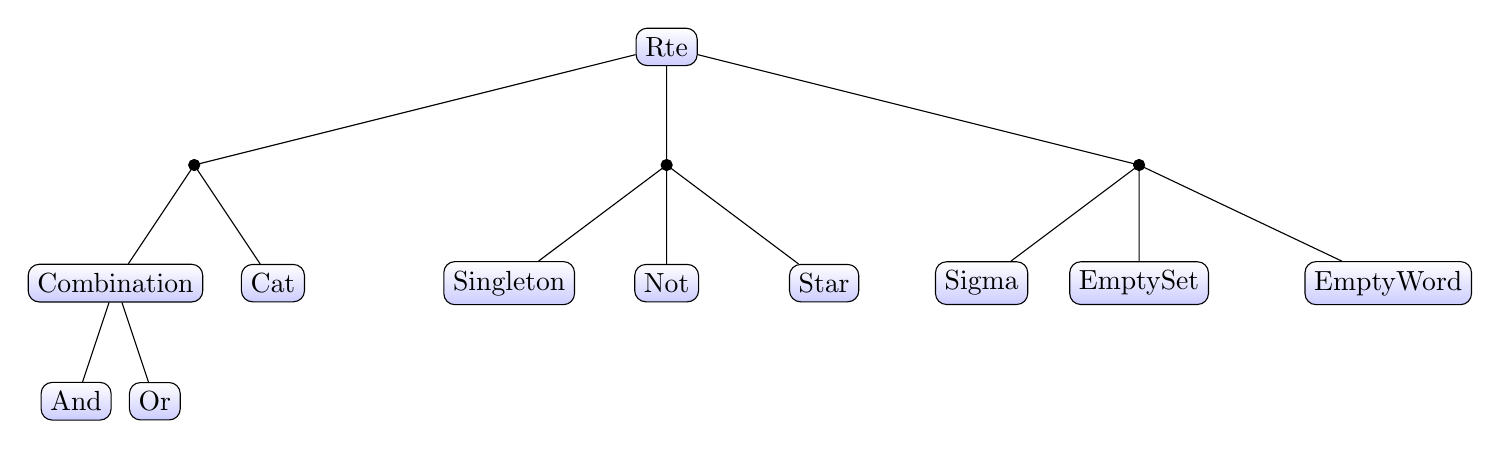
\begin{tikzpicture}[sibling distance=10em,
  every node/.style = {shape=rectangle, rounded corners,
    draw, align=center,
    top color=white, bottom color=blue!20}]]
    \tikzstyle{level 1}=[sibling distance=60mm]
    \tikzstyle{level 2}=[sibling distance=20mm]
    \tikzstyle{level 3}=[sibling distance=10mm]
  \node {Rte}
    child { [fill] circle (2pt)
      child { node {Combination} 
        child { node {And} }
        child { node {Or} } }
      child { node {Cat} } }
    child { [fill] circle (2pt)
      child { node {Singleton} }
      child { node  {Not} }
      child { node {Star} } }
    child { [fill] circle (2pt)
      child { node {Sigma} }
      child { node {EmptySet} }
      child { node [right=1mm] {EmptyWord} } } ;
\end{tikzpicture}
\end{document}
